\section{Probability Theory} \label{sec:Probability Theory}
There are 3 main components to \nameref{sec:Probability Theory}.
\begin{enumerate}[noitemsep, nolistsep]
	\item \nameref{sec:Set Theory}
	\item \nameref{subsec:Probability Law Corollary}
	\item \nameref{subsec:Conditional Probability}~and~\nameref{subsec:Event Independence}
\end{enumerate}

	\subsection{Random Experiments} \label{subsec:Random Experiments}
	\begin{definition}[Random Experiment] \label{def:Random Experiment}
		A \emph{random experiment} is an experiment whose outcome varies in an unpredictable fashion when performed under the same conditions.
	\end{definition}
	\begin{definition}[Sample Space] \label{def:Sample Space}
		A \emph{sample space, $S$} of a random experiment is the set of all possible experiments' outcomes.
	\end{definition}
	\begin{definition}[Outcome/Sample Point] \label{def:Outcome}
		An \emph{outcome}, or \emph{sample point} of a random experiment is a result that cannot be decomposed into other results.
	\end{definition}
	\begin{definition}[Event] \label{def:Event}
		An \emph{event} corresponds to a subset of the sample space. We say an event occurs if and only if (iff) the outcome of the experiment is in the subset representing the event.
	\end{definition}
	\begin{definition}[Event Classes] \label{def:Event Classes}
		An \emph{event class} $\EventClass$ is the collection of the all the events' sets. $\EventClass$ should be closed under unions, intersections, and complements.
		\begin{itemize}[noitemsep, nolistsep]
			\item For $S$ finite, or countably infinite, then we can let $\EventClass$ be all subsets of $S$.
			\item For $S$ uncountably infinite, instead we can let $\EventClass$ consist of the subsets that can be obtained as countable unions and intersections of some sets of $\EventClass$.
		\end{itemize}
	\end{definition}
	\begin{definition}[Probability Law] \label{def:Probability Law}
		A \emph{probability law} for a random experiment $E$, with sample space $S$, and an event class $\EventClass$ is a rule that assigns to each event $A \in \EventClass$ a number $P \left[A \right]$, called the probability of $A$ that satisfies the axioms:
		\begin{enumerate}[label=Axiom~\Roman*:, align=left, noitemsep, nolistsep] \label{subdef:Probability Law Axioms}
			\item $0 \leq P\left[ A \right]$
			\item $P \left[ S \right] = 1$
			\item If $A \cap B = \emptyset$, then $P \left[ A \cup B \right] = P \left[ A \right] + P \left[ B \right]$
			\item[Axiom III':] If $A_{1}$, $A_{2}$, $\ldots$ is a sequence of events such that $A_{i} \cap A_{j} = \emptyset$ for all $i \neq j$, then $P \left[ \bigcup_{k=1}^{\infty} A_{k} \right] = \sum_{k=1}^{\infty} P \left[ A_{k} \right]$
		\end{enumerate}
	\end{definition}
	
	\subsection{Probability Law Corollaries} \label{subsec:Probability Law Corollary}
		\begin{enumerate}[label=Axiom~\Roman*:, align=left, noitemsep, nolistsep] % Probability Law Axioms
			\item $0 \leq P\left[ A \right]$
			\item $P \left[ S \right] = 1$
			\item If $A \cap B = \emptyset$, then $P \left[ A \cup B \right] = P \left[ A \right] + P \left[ B \right]$
			\item[Axiom III':] If $A_{1}$, $A_{2}$, $\ldots$ is a sequence of events such that $A_{i} \cap A_{j} = \emptyset$ for all $i \neq j$, then $P \left[ \bigcup_{k=1}^{\infty} A_{k} \right] = \sum_{k=1}^{\infty} P \left[ A_{k} \right]$
		\end{enumerate}
		\begin{corollary} \label{cor:Probability Parts}
			$P \left[ A^{C} \right] = 1 - P \left[ A \right]$
		\end{corollary}
		\begin{corollary} \label{cor:Probability of Event}
			$P \left[ A \right] \leq 1$
		\end{corollary}
		\begin{corollary} \label{cor:Probability of Empty Set}
			$P \left[ \emptyset \right] = 0$
		\end{corollary}
		\begin{corollary} \label{cor: Probability Addition of Disjoint Pairs}
			If $A_{1}$, $A_{2}$, $\ldots$, $A_{n}$ are pairwise mutually exclusive ($A_{1} \cap A_{2} \cap \ldots \cap A_{n} = \emptyset$), then $P \left[ \bigcup_{k=1}^{n} \right] = \sum_{k=1}^{n} P \left[ A_{k} \right]$ for $n \geq 2$
		\end{corollary}
		\begin{corollary} \label{cor:Inclusion-Exclusion Principle to 2 Sets}
			$P \left[ A \cup B \right] = P \left[ A \right] + P \left[ B \right] - P \left[ A \cap B \right]$
		\end{corollary}
		\begin{corollary} \label{cor:Inclusion-Exclusion Principle to n Sets}
			$P \left[ A \cup B \right] = \sum\limits_{j=1}^{n} P \left[ A_{j} \right] - \sum_{j<k} P \left[A_{j} \cap A_{k} \right] + \ldots + \left( -1 \right)^{n+1} P \left[ A_{1} \cap \ldots \cap A_{n} \right]$
		\end{corollary}
		\begin{corollary} \label{cor:Subset Probability to Superset}
			If $A \subset B$, then $P \left[ A \right] \leq P \left[ B \right]$
		\end{corollary}
	
	\subsection{Conditional Probability} \label{subsec:Conditional Probability}
		\begin{definition}[Conditional Probability] \label{def:Conditional Probability}
			The \emph{conditional probability} of event $A$ \textbf{GIVEN THAT} event $B$ occurred is denoted $P \left[ A \vert B \right]$ and is defined as
			\begin{equation} \label{eq:Conditional Probability}
				P \left[ A \vert B \right] = \frac{P \left[ A \cap B \right]}{P \left[ B \right]}
			\end{equation}
		\end{definition}
		\begin{theorem}[Theorem of Total Probability] \label{thm:Theorem of Total Probability}
			Let $B_{1}$, $B_{2}$, $\ldots$, $B_{n}$ be mutually exclusive events whose union equals the sample space $S$, i.e. $B_{1}$, $B_{2}$, $\ldots$, $B_{n}$ is a partition of $S$.
		\end{theorem}
		\begin{definition}[Baye's Rule] \label{def:Baye's Rule}
			Let $B_{1}$, $B_{2}$, $\ldots$, $B_{n}$ be a partition of sample space $S$.
			\begin{equation}
				P \left[ B_{j} \vert A \right] = \frac{P \left[ A \cap B_{j} \right]}{P \left[ A \right]}
				= \frac{P \left[ A \vert B_{j} \right] * P \left[ B_{j} \right]}{\sum\limits_{k=1}^{n} P \left[ A \vert B_{k} \right] * P \left[ B_{k} \right]}
			\end{equation}
		\end{definition}
		\begin{example}[Exam 1, Problem 5]{Baye's Rule}
			An urn contains 9 balls, identical in every way, except that they are labeled with numbers 1 through 9.
			Two balls are selected at random, without replacement, and the sequence of labels observed are recorded.
			\begin{boldalphlist}
				\item Give the formula for the conditional probability of event $A$ given that event $B$ occurred (where $A$ and $B$ are arbitrary events).
				\item What is the probability that the label of the second ball is even?
				\item What is the probability that the label of the first ball was odd given that the second was even?
			\end{boldalphlist}
		
			\tcblower
			To begin, it is usually best if you create an event tree, like below.
			\newline
			\begin{center}
				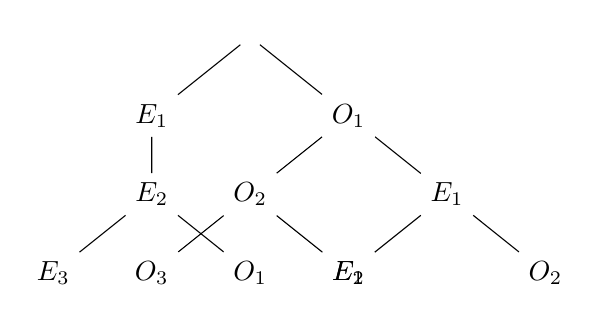
\begin{tikzpicture}[level distance=1.0cm,
nodes={align=center},sibling distance=25mm]

% Nodes
\node{}
	child{node{$E_{1}$} % First Draw Option 1
		child{node{$E_{2}$}
			child{node{$E_{3}$}}
			child{node{$O_{1}$}}
		}
%		child{node{$O_{1}$}
%			child{node{$O_{2}$}}
%			child{node{$E_{2}$}}
%		}
	}
	child{node{$O_{1}$} % First Draw Option 2
		child{node{$O_{2}$}
			child{node{$O_{3}$}}
			child{node{$E_{1}$}}
		}
		child{node{$E_{1}$}
			child{node{$E_{2}$}}
			child{node{$O_{2}$}}
		}
	};

\end{tikzpicture}
			\end{center}
			\begin{enumerate}[label=(\alph*)]
				\item $\Prob \left[ A \Given B \right] = \frac{\Prob \left[ A \cap B \right]}{\Prob \left[ B \right]}$
				\item 
			\end{enumerate}
		\end{example}
	
	\subsection{Event Independence} \label{subsec:Event Independence}
		\begin{definition}[Independent] \label{def:Event Independence}
			Two events $A$ and $B$ are \emph{independent} if 
			\begin{equation} \label{eq:Event Independence}
				P \left[ A \cap B \right] = P \left[ A \right] * P \left[ B \right], P\left[ A \right] \neq 0, P\left[ B \right] \neq 0
			\end{equation}
			\begin{itemize}[noitemsep, nolistsep]
				\item If $A \cap B = \emptyset$, the $A$ and $B$ are \textbf{dependent}.
				\item If checking for independence between more than 2 events, you must check each pair, each triple, etc. until you check the independence of each event against each other. For 3 events, $A$, $B$, $C$:
					\begin{itemize}[noitemsep, nolistsep]
						\item Check $P \left[ A \cap B \cap C \right] = P \left[ A \right] * P \left[ B \right] * P \left[ C \right]$
						\item Also need to check:
							\begin{enumerate}[noitemsep, nolistsep]
								\item $P \left[ A \cap B \right] = P \left[ A \right] * P \left[ B \right]$
								\item $P \left[ B \cap C \right] = P \left[ B \right] * P \left[ C \right]$
								\item $P \left[ A \cap C \right] = P \left[ A \right] * P \left[ C \right]$
							\end{enumerate}
					\end{itemize}
			\end{itemize}
		\end{definition}
		\begin{example}[Exam 1, Problem 4]{Event Independence}
			Let $S=\lbrace 1,2,3,4 \rbrace$, and $A = \lbrace 1,2 \rbrace$, $B=\lbrace 1,3 \rbrace$, $C = \lbrace 1,4 \rbrace$, $D = \lbrace 3,4 \rbrace$.
			Assume the outcomes are equiprobable.
			Are the following events independent?
				\begin{enumerate}[noitemsep, nolistsep]
					\item $A$ and $B$
					\item $A$ and $D$
					\item $A$, $B$, and $C$
				\end{enumerate}
		\end{example}
	If 2 events $A$ and $B$ are independent, then their complements are also independent. This is shown in \nameref{proof:Independence of Complements of Events}.
		\begin{proof}[Independence of Complements of Events] \label{proof:Independence of Complements of Events}
			We assumed that $A$ and $B$ were independent, so $P \left[ A \cap B \right] = P \left[ A \right] \cdot P \left[ B \right]$.
			There are 2 more facts we will need:
			\begin{enumerate}[leftmargin=1.0in, label=Fact \arabic*: , ref=Fact \arabic*, noitemsep, nolistsep]
				% leftmargin sets a distance for left margin
				% ref sets the way items will be cross-referenced, and can differ from the label.
				\item $P \left[ B \right] + P \left[ B^{C} \right] = 1$ \label{proof:Independence of Complements of Events:Fact 1}
				\item $P \left[ A \cap B^{C} \right] + P \left[ A \cap B \right] = P \left[ A \right]$ \label{proof:Independence of Complements of Events:Fact 2}
			\end{enumerate}
			From \ref{proof:Independence of Complements of Events:Fact 1}, we have:
			\begin{equation*}
				P \left[ A \cap B \right] = P \left[ A \right] \cdot \left( 1-P \left[ B^{C} \right] \right)
			\end{equation*}
			From \ref{proof:Independence of Complements of Events:Fact 2}, we have $P \left[ A \cap B \right] = P \left[ A \right] - P \left[ A \cap B^{C} \right]$.
			Substituting these into the equation above:
			\begin{align*}
				P \left[ A \right] - P \left[ A \cap B^{C} \right] &= P \left[ A \right] \cdot \left( 1-P \left[ B^{C} \right] \right)\\
				P \left[ A \right] - P \left[ A \cap B^{C} \right] &= P \left[ A \right] - P \left[ A \right] \cdot P \left[ B^{C} \right] \\
				- P \left[ A \cap B^{C} \right] &= -P \left[ A \right] \cdot P \left[ B^{C} \right] \\
				P \left[ A \cap B^{C} \right] &= P \left[ A \right] \cdot P \left[ B^{C} \right] \\
			\end{align*}
			$\therefore$ $A$ and $B^{C}$ are independent, according to the definition of \nameref{def:Event Independence}~events in \Cref{eq:Event Independence}.
		\end{proof}
%%% Local Variables:
%%% mode: latex
%%% TeX-master: "../Math_374-Reference_Sheet"
%%% End:
